%==============================================================================%
%==========================|     CHAPTER 3 Method    |=========================%
%==============================================================================%
\chapter{Proposed Method} \label{chap:Method}
This chapter outlines the systematic approach used to evaluate the selected open-source Breach and Attack Simulation (BAS) tools. It focuses on creating a repeatable, evidence-based assessment of each tool’s usability and effectiveness. The methodology unfolds in four phases: establishing the conceptual framework, justifying the selection of MITRE Caldera, Infection Monkey, and Atomic Red Team, mapping their features in a comparison matrix, and finally, applying a scoring system to grade critical metrics like installation complexity and reporting quality.

%--------------------|    3.1 Conceptual Framework    |--------------------------------|
\section{Conceptual Framework}\label{sec:conceptual_framework}
To ensure a fair, systematic, and methodologically sound assessment of open-source Breach and Attack Simulation (BAS) tools, this study is governed by a structured conceptual framework (showed in Figure~\ref{fig:research_workflow}). This framework is specifically designed to isolate key variables, maintain consistent environmental factors, and guarantee the production of reliable and repeatable results across all tool deployments and test executions.

\begin{figure}
    \centering
    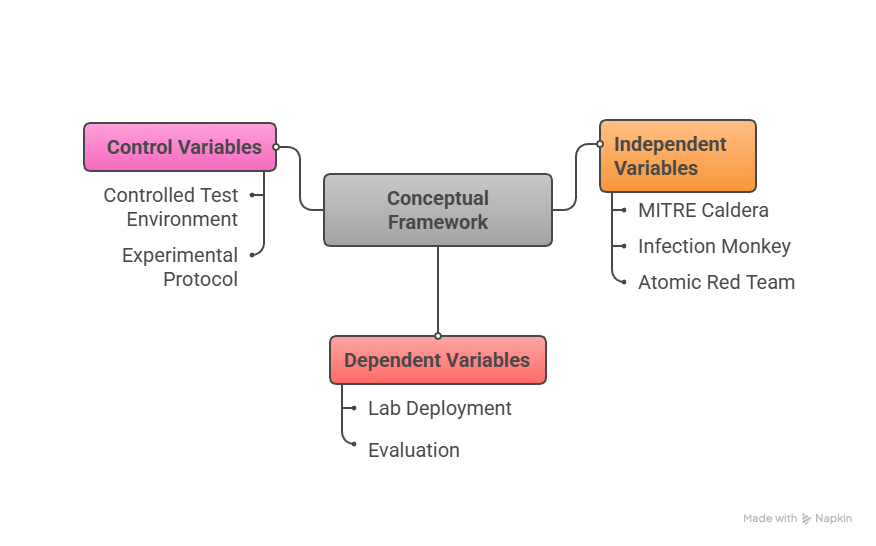
\includegraphics[width=1\textwidth]{figures/Conceptual Framework.png}
    \caption{Conceptual Framework of the Study}
    \label{fig:research_workflow}
\end{figure}

Figure~\ref{fig:research_workflow} displays the overall workflow for this comparative study outlined as follows:

\begin{itemize}
    \item \textbf{Independent Variables:} The core element under examination, which is the set of open-source BAS tools selected for comparative evaluation. This variable consists of three distinct solutions: MITRE Caldera, Infection Monkey, and Atomic Red Team. The study’s aim is to observe the performance differences resulting from the deployment of these tools within the controlled experimental environment.
    \item \textbf{Dependent Variables:} Represent the measurable outcomes resulting from the implementation of the independent variable, segmented into two primary categories. The first category, \textit{Lab Deployment}, captures the essential setup parameters for each tool, including the hardware baseline, the specific operating system and software version used, and the established endpoint count for the simulation. The second category, \textit{Evaluation Metrics}, focuses on quantifiable assessment criteria: Installation complexity, Performance, Reporting capabilities, and Content update frequency.
    \item \textbf{Control Variables:} To ensure the validity and reproducibility of the results, the study strictly maintains a set of Control Variables designed to eliminate confounding factors and external bias. These controls are grouped into two key areas:
    
    \begin{enumerate}
        \item \textbf{Controlled Test Environment:} This ensures that all tools operate under identical infrastructure conditions, specifically using identical hardware specifications, uniform agent/server images, and consistent network access across all test runs.
        
        \item \textbf{Experimental Protocol:} This maintains procedural consistency by employing predefined attack use cases, conducting repeated attack simulations, utilizing a unified comparison matrix for feature mapping, and applying a consistent scoring rubric for objective metric assessment.
    \end{enumerate}
 \end{itemize}   
 
\textbf{Research Workflow}
    \begin{enumerate}
        \item Select open-source BAS tools (MITRE Caldera, Infection Monkey, Atomic Red Team).
        \item Propose and define six distinct comparison metrics for evaluation.
        \item Prepare standardized experimental environments using uniform virtual machine configurations.
        \item Install and configure each BAS tool according to its documentation.
        \item Design testing scenarios mapped to MITRE ATT\&CK techniques.
        \item Execute attack simulations for each selected tool.
        \item Capture output data and performance results.
        \item Evaluate each BAS tool against the six metrics.
        \item Aggregate findings and visualize the comparative results using a radar chart to highlight relative strengths and weaknesses in a multi-dimensional view.
    \end{enumerate}

\begin{figure}
    \centering
    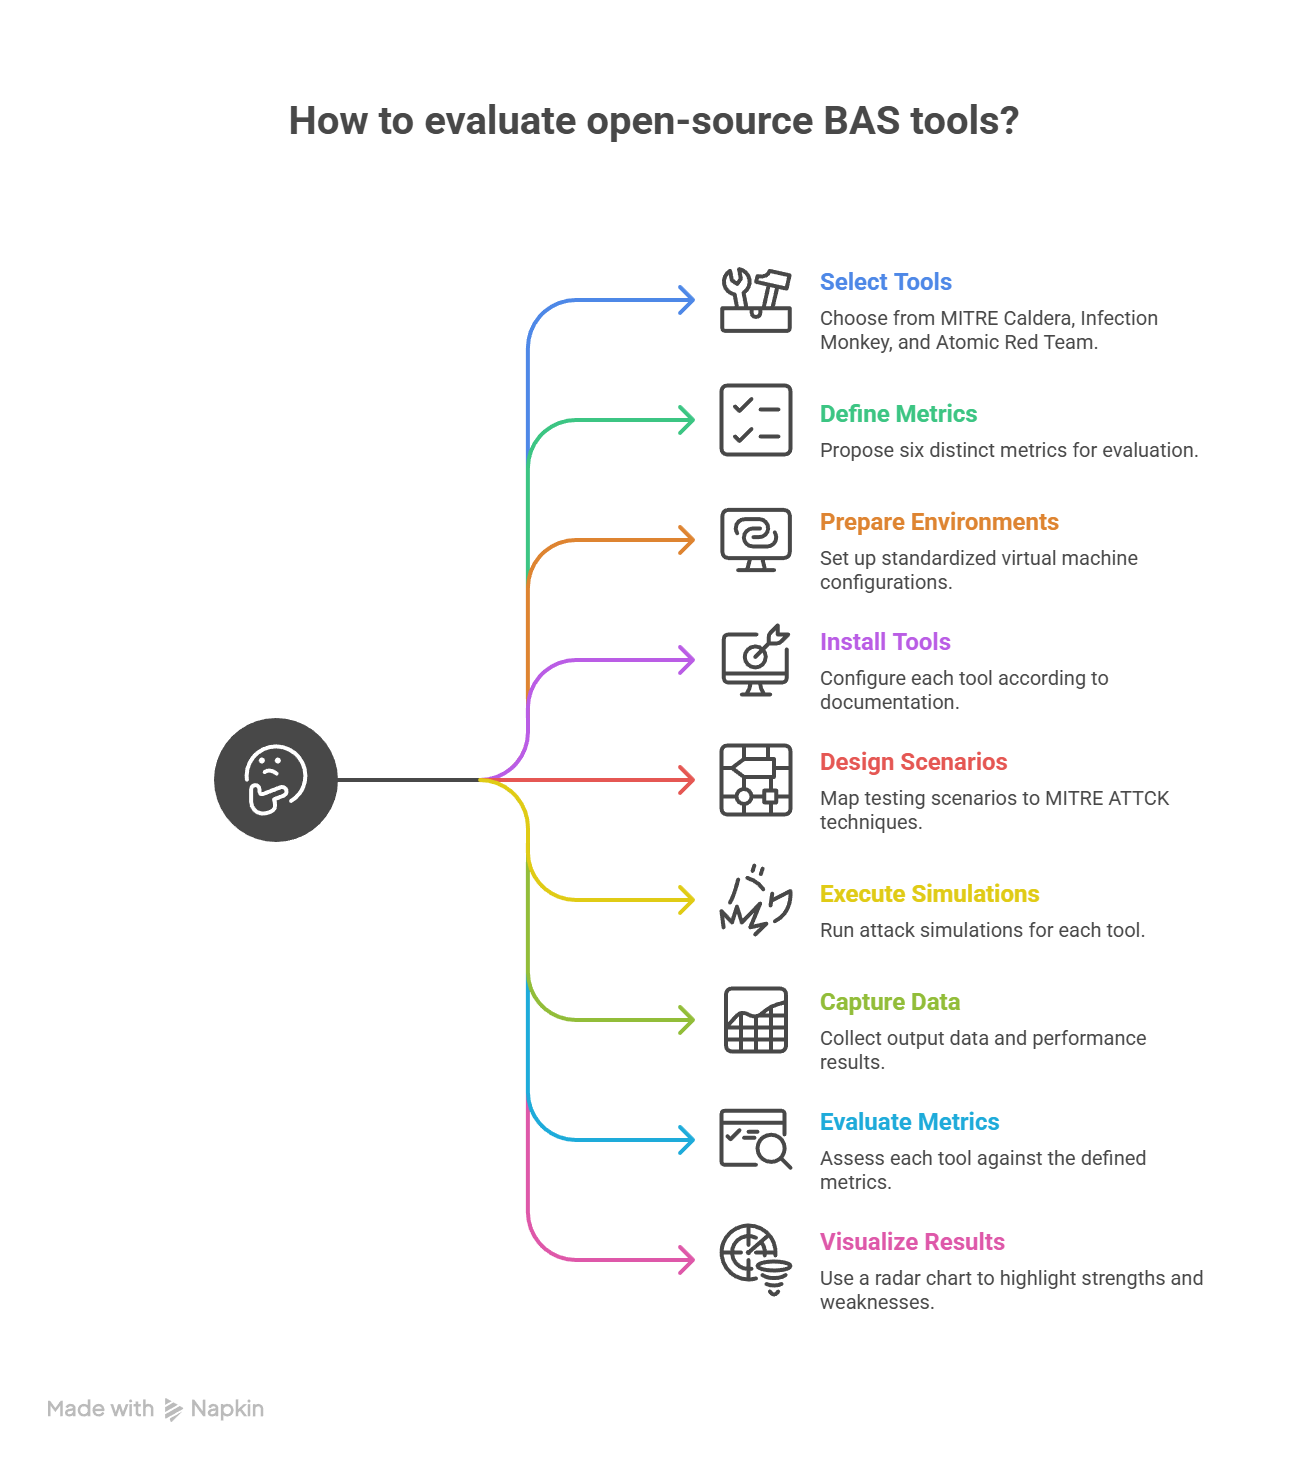
\includegraphics[width=1\linewidth]{figures/BAS-Research Workflow.png}
    \caption{Research Workflow}
    \label{fig:BAS-Research Workflow}
    \end{figure}

%--------------------|    3.2 Selection of Open-Source BAS Solutions    |-----------------------|
\section{Selection of Open-Source BAS Solutions}
The selection process for this research employed a systematic \textbf{down-selection methodology} to ensure the chosen candidates represent the "gold standard" of modern open-source Breach and Attack Simulation (BAS). The process was executed in two distinct phases. Phase 1 applied binary architectural criteria—automation capability, repository health, and MITRE ATT\&CK framework alignment—to remove tools incompatible with autonomous laboratory deployment. Phase 2 applied a weighted AI consensus ranking to confirm the selection of the three highest-quality candidates for physical laboratory testing.

\subsection{Phase 1: Scope Filtering (Binary Exclusion)}
This study began with the nine tools identified in the foundational work of Landauer et al. ~\cite{landauer2024}. To isolate platforms suitable for a high-fidelity laboratory environment, three \textbf{Inclusion Criteria} were applied to assess architectural viability:

\begin{itemize}
    \item \textbf{Automation Capability:} The tool must support autonomous, multi-stage attack emulation—where subsequent actions depend on the success of previous steps—rather than static infection simulation or manual per-step execution.
    \item \textbf{Active Repository Health:} The tool must have received community updates within the last 36 months to ensure compatibility with modern, patched Linux environments (specifically Ubuntu 22.04/24.04 LTS and recent Kernel versions).
    \item \textbf{Framework Alignment:} The tool must natively map its procedures to the MITRE ATT\&CK framework to ensure standardized, industry-relevant reporting.
\end{itemize}

\begin{figure}[htbp]
    \centering
    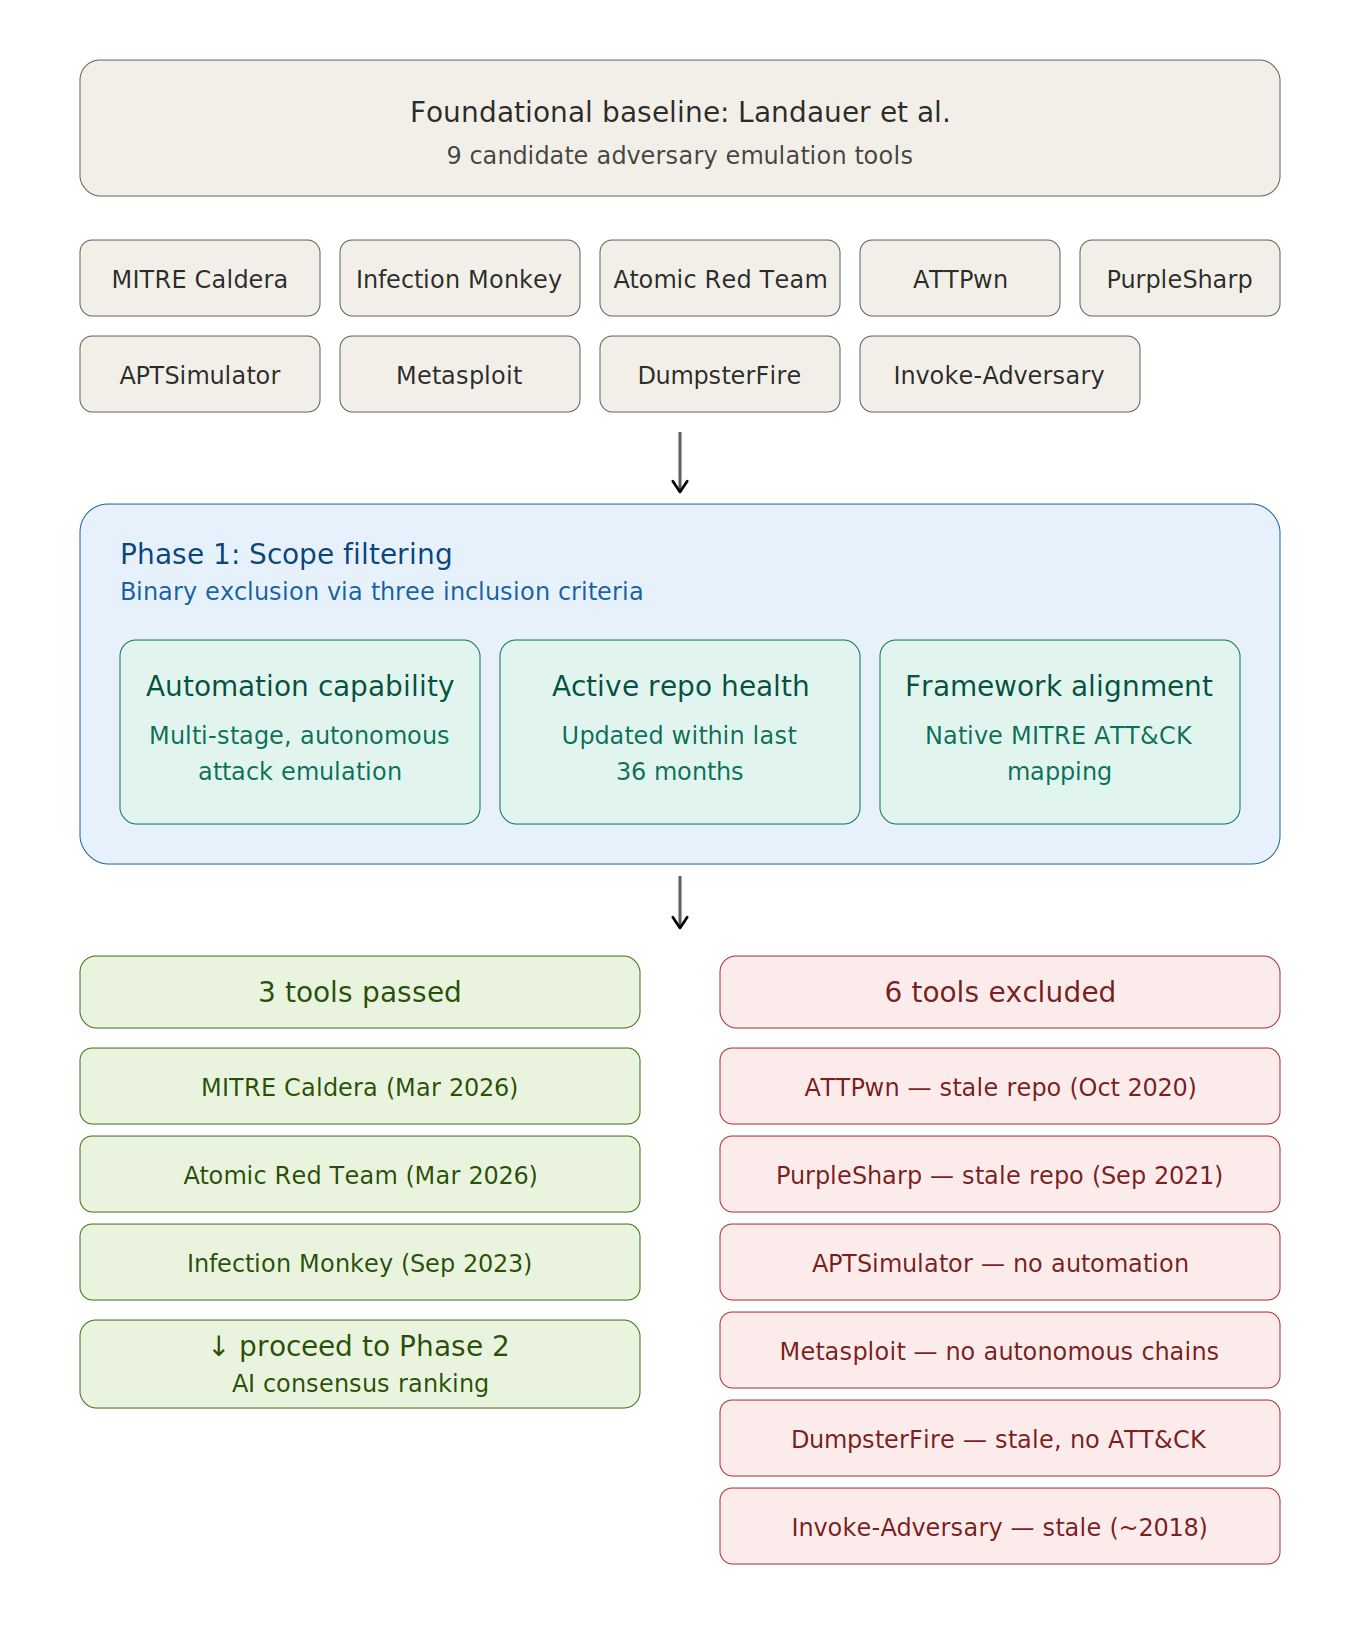
\includegraphics[width=1\linewidth]{figures/phase_1_scope_filtering.png}
    \caption{Scope filtering via binary exclusion.}
    \label{fig:Selection_phase1}
\end{figure}

As shown in Figure~\ref{fig:Selection_phase1}, application of the three criteria produced a clean partition of the candidate pool. The binary evaluation and current repository health of the initial tool pool are summarized in Table~\ref{tab:phase1_checklist}.

\begin{table}
    \centering
    \caption{Binary selection matrix for open-source BAS tools (Status: March 2026)}
    \label{tab:phase1_checklist}
    \renewcommand{\arraystretch}{1.4}
    \begin{tabular}{|l|c|c|c|c|c|}
        \hline
        \textbf{Tool Candidate} & \textbf{Automation} & \textbf{Repo Health} & \textbf{Last Update} & \textbf{Framework} & \textbf{Result} \\ \hline
        \textbf{MITRE Caldera}    & [Yes] & [Yes] & Mar 2026 & [Yes] & \textbf{PASS} \\ \hline
        \textbf{Infection Monkey} & [Yes] & [Yes] & Sep 2023 & [Yes] & \textbf{PASS} \\ \hline
        \textbf{Atomic Red Team}  & [Yes] & [Yes] & Mar 2026 & [Yes] & \textbf{PASS} \\ \hline
        ATTPwn                    & [Yes] & [No]  & Oct 2020 & [Yes] & FAIL \\ \hline
        PurpleSharp               & [Yes] & [No]  & Sep 2021 & [Yes] & FAIL \\ \hline
        APTSimulator              & [No]  & [Yes] & Jul 2023 & [Yes] & FAIL \\ \hline
        Metasploit                & [No]  & [Yes] & Mar 2026 & [Yes] & FAIL \\ \hline
        DumpsterFire              & [Yes] & [No]  & Dec 2017 & [No]  & FAIL \\ \hline
        Invoke-Adversary          & [Yes] & [No]  & $\sim$2018 & [Yes] & FAIL \\ \hline
    \end{tabular}
\end{table}

\noindent \textbf{Technical Justification for Inclusion:}
The following three tools—MITRE Caldera, Infection Monkey, and Atomic Red Team—successfully met all criteria. These platforms demonstrate the necessary architectural depth for empirical performance measurement on Ubuntu systems, supporting autonomous decision-making and active alignment with the MITRE ATT\&CK matrix.

\noindent \textbf{Technical Justification for Exclusion:}
Six tools were excluded due to specific architectural or maintenance limitations identified in Table~\ref{tab:phase1_checklist}:
\begin{itemize}
    \item \textbf{ATTPwn (Failed Repo Health):} Stagnant since October 2020. The repository is considered legacy and lacks the necessary updates to support modern MITRE ATT\&CK technique variations or current Ubuntu-based Python dependencies.
    \item \textbf{PurpleSharp (Failed Repo Health):} No significant updates since late 2021, exceeding the 36-month maintenance threshold. It relies on legacy .NET assemblies that exhibit limited compatibility with modern security orchestration requirements.
    \item \textbf{APTSimulator (Failed Automation):} Functions as a "static artifact creator" that drops fake registry keys and files; it does not execute real-time network traffic or process-level behaviors required for dynamic telemetry.
    \item \textbf{Metasploit (Failed Automation):} Although powerful, it is a manual penetration testing framework requiring human-in-the-loop operation; it lacks the autonomous planning engine required for automated BAS research.
    \item \textbf{DumpsterFire (Failed Health/Alignment):} Stagnant since 2017. It lacks native MITRE ATT\&CK mapping and exhibits significant dependency rot on modern Ubuntu kernels.
    \item \textbf{Invoke-Adversary (Failed Repo Health):} No significant updates in over 8 years. The repository is functionally incompatible with modern Ubuntu Python and PowerShell Core environments.
\end{itemize}

This filtering phase resulted in three primary candidates, which were then subjected to Phase 2 comparative ranking.

\subsection{Phase 2: Selection via AI Consensus Ranking (Weighted Evaluation)}
To finalize the selection, a triangulated AI evaluation was conducted using five independent artificial intelligence (AI) assistants: Gemini, ChatGPT, Copilot, Claude, and DeepAI. These models were tasked with ranking the three Phase 1 survivors against open-ended write-in alternatives, based on industry adoption, scenario extensibility, and documentation quality, as of May 2026. This open-ended formulation was deliberate: it allowed contemporary platforms outside the Landauer et al. baseline to surface as write-in candidates, providing a transparency check on whether any modern BAS tool had been overlooked by the foundational baseline.

\begin{figure}
    \centering
    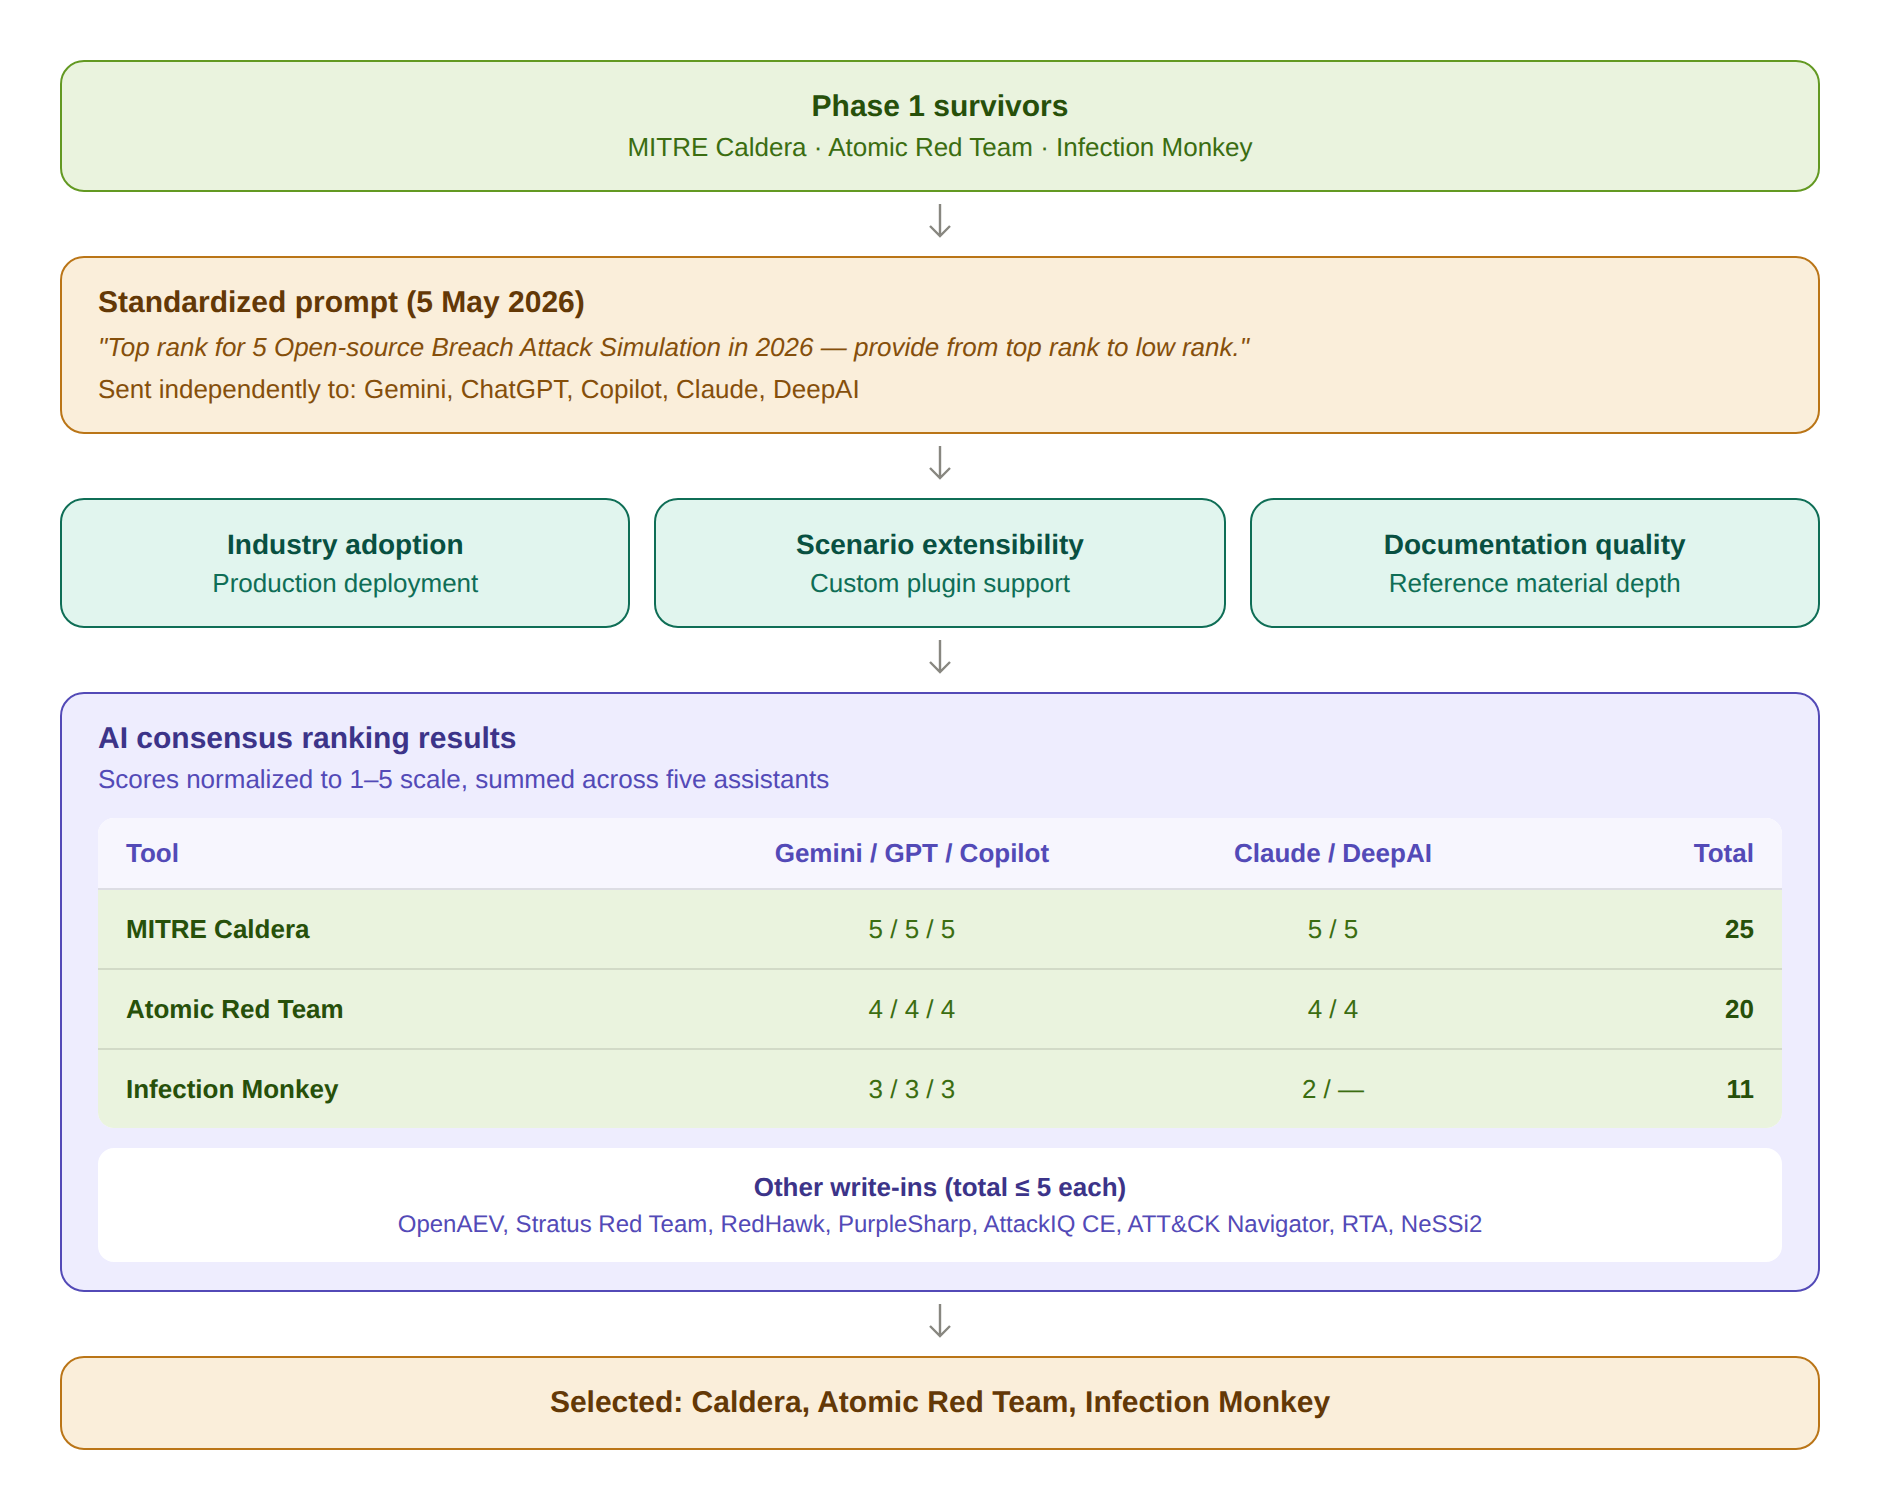
\includegraphics[width=1\linewidth]{figures/Select_Phase2.png}
    \caption{AI consensus ranking via weighted triangulation.}
    \label{fig:Selection_phase2}
\end{figure}

As showed in Figure~\ref{fig:Selection_phase2}, a point-based scoring system was applied (1st place = 5 points, 2nd place = 4 points, 3rd place = 3 points, etc.) to synthesize the rankings and mitigate individual model bias. The results of this process, summarized in Table~\ref{tab:bas_consensus}, consistently identified MITRE Caldera, Atomic Red Team, and Infection Monkey as the most highly ranked platforms.

\begin{table}
\centering
\caption{AI consensus ranking of open-source BAS candidates (5 May 2026)}
\label{tab:bas_consensus}
\renewcommand{\arraystretch}{1.25}
\begin{tabular}{l c c c c c >{\columncolor{lightgray}}c}
\toprule
\textbf{Tool Candidate} & \textbf{Gemini} & \textbf{ChatGPT} & \textbf{Copilot} & \textbf{Claude} & \textbf{DeepAI} & \textbf{Total Score} \\
\midrule
\textbf{MITRE Caldera}     & 5 & 5 & 5 & 5 & 5  & \textbf{25} \\
\textbf{Atomic Red Team}   & 4 & 4 & 4 & 4 & 4  & \textbf{20} \\
\textbf{Infection Monkey}  & 3 & 3 & 3 & 2 & -- & \textbf{11} \\
\midrule
OpenAEV            & 2  & -- & -- & 3  & -- & \textbf{5} \\
Stratus Red Team   & 1  & 2  & -- & 1  & -- & \textbf{4} \\
RedHawk            & -- & -- & -- & -- & 3  & \textbf{3} \\
PurpleSharp        & -- & -- & -- & -- & 2  & \textbf{2} \\
AttackIQ CE        & -- & -- & 2  & -- & -- & \textbf{2} \\
ATT\&CK Navigator  & -- & -- & -- & -- & 1  & \textbf{1} \\
RTA                & -- & 1  & -- & -- & -- & \textbf{1} \\
NeSSi2             & -- & -- & 1  & -- & -- & \textbf{1} \\
\bottomrule
\end{tabular}
\end{table}

Several write-in candidates were proposed by individual assistants, most notably OpenBAS/OpenAEV (rebranded by Filigran in November 2025), alongside Metasploit, Stratus Red Team, Prelude Operator, Purple Sharpie, AttackIQ, Red Team Tools, and Scythe. None of these accumulated more than four points across the panel, falling well short of the lowest-ranked Phase 1 survivor (Infection Monkey at 13 points). This substantial gap between the three Phase 1 survivors and the write-in tier provides triangulated validation that the foundational baseline of Landauer et al. continues to enclose the most defensible open-source BAS candidates as of April 2026.

\subsection{Selection Summary}
The triangulation process produced a clear hierarchy that was consistent across both phases. \textbf{MITRE Caldera} emerged as the primary candidate due to its sophisticated "Abilities and Adversaries" engine, which provides the deepest support for autonomous, multi-stage attack chains. \textbf{Atomic Red Team} was selected as the second-ranked platform, serving as the industry-standard library for atomic test execution and offering the broadest community-maintained ATT\&CK technique coverage. \textbf{Infection Monkey} was selected as the third candidate for its unique focus on automated lateral movement and network resilience testing, complementing the procedural depth of the other two platforms. Together, these three tools form the basis of the subsequent empirical evaluation in this research.

%-------------------------------|    3.3 Comparison matrix    |---------------------------------|
\section{Comparison Matrix}
To ensure the evaluation framework is both grounded in established academic standards and capable of addressing the critical research gaps identified in Chapter~2, the assessment of each open-source BAS tool is based on six criteria. The framework adopts a hybrid approach: several criteria are adapted directly from existing literature, while others are introduced by this study to measure practical operational realities that previous theoretical models omitted. The justification for each criterion is defined as follows:

\begin{enumerate}
    \item \textbf{Usability \& Deployment Complexity:} This criterion evaluates tool implementation friction by quantifying required installation steps and package dependencies. Addressing the high deployment complexity that often hinders open-source adoption, this criterion operationalizes the Installation \& Configuration category from Landauer et al.~\cite{landauer2024} into exact, laboratory-measured deployment parameters.

    \item \textbf{Threat Intelligence Alignment \& Maintenance:} This criterion assesses the frequency and automation of repository updates. Because stagnant tools quickly lose validation value against evolving threats, this criterion operationalizes the requirement for dynamic scenario feedback established by Wang et al.~\cite{wang2025} into a measurable assessment of how effectively a tool modernizes its attack library.

    \item \textbf{Scenario Coverage, Reliability \& Relevance:} This criterion adapts elements of the Features \& Capabilities category from Landauer et al.~\cite{landauer2024} (such as mapping to MITRE ATT\&CK) and integrates the necessity for multi-stage attack modeling established by Kuhl et al.~\cite{kuhl2007}. In addition, this study introduces an empirical reliability test that, to the author's knowledge, has not previously been applied to comparative evaluation of open-source BAS tools. Rather than relying on qualitative offline checklists or synthetic data, the introduced sub-criterion evaluates the tool's library alignment, indexed in this study as S1 through S20, and its empirical execution success rate in a live laboratory environment to ensure payloads run without crashing the target system.

    \item \textbf{Operational Performance \& Output Quality:} Previous academic models~\cite{wang2025,kuhl2007} did not address the computational cost of running simulation infrastructure. This study therefore introduces a performance criterion that records the BAS server's exact resource overhead (CPU and RAM) during active simulation. To isolate variables, execution is verified solely via native operating-system telemetry (e.g., Windows Event Logs, auditd). The criterion further evaluates the actionable quality of each tool's security reports, drawing on Roque et al.~\cite{roque2024}'s demonstration that report quality directly determines the value of simulation outcomes for downstream defensive tuning.

    \item \textbf{Framework Extensibility \& Custom Scenario Creation:} This criterion evaluates the technical difficulty of customizing TTPs or modifying attack chains. Grounded in the theoretical frameworks of Wang et al.~\cite{wang2025} and adapting specific elements from Landauer et al.~\cite{landauer2024}'s Features \& Capabilities category, it measures the tool's capacity to emulate highly specific, industry-relevant threat actors by quantifying the technical friction of custom payload creation (e.g., GUI/YAML editing versus core programming).

    \item \textbf{Community Health \& Project Maturity:} This criterion evaluates long-term project viability by measuring commit frequency and GitHub community metrics. Since open-source tools rely entirely on volunteer maintainers, abandoned projects pose significant operational risks. Adapted from the Community \& Support category of Landauer et al.~\cite{landauer2024}, this criterion translates qualitative community assessments into objective evaluations utilizing public repository data.
\end{enumerate}

By synthesizing existing literature with these new operational measurements, the resulting evaluation framework — operationalized in Section~\ref{sec:Scoring} as the Complete Evaluation Scoring Matrix (Table~\ref{tab:bas_evaluation_matrix_complete}) — facilitates a comprehensive, real-world assessment of each tool's capabilities.

%--------------------------------|    3.4 Comparison Matrix    |--------------------------------|
\section{Evaluation Scoring Matrix}\label{sec:Scoring}
This matrix provides a detailed breakdown of the scoring for each evaluation criterion on a 0–3 scale, enabling a clear and quantitative comparison of the open-source BAS tools. Scores are derived either from direct Experimental Data (Exp) gathered during laboratory simulations, or through Document and Online Searches (Search) for metrics evaluating project maturity. The final comparative results will be visually represented using a spider chart, illustrating the performance of each tool across the six metrics.


%###############| Complete Evaluation Scoring Matrix |##################
\begin{longtable}{|l|p{4cm}|p{8cm}|l|}
    \caption{Complete Evaluation Scoring Matrix}
    \label{tab:bas_evaluation_matrix_complete} \\
    \hline
    \textbf{ID} & \textbf{Criterion Description} & \textbf{Scoring Scale} & \textbf{Src} \\
    \hline
    \endfirsthead
    \hline
    \textbf{ID} & \textbf{Criterion Description} & \textbf{Scoring Scale} & \textbf{Src} \\
    \hline
    \endhead
    
    % --- SECTION 1 ---
    \multicolumn{4}{|l|}{\textbf{1. Usability \& Deployment Complexity}} \\
\hline
    1.1 & Number of installation steps required ~\cite{landauer2024} & 
    [3] Very Simple ($<$ 6 steps) \newline 
    [2] Standard (6--10 steps) \newline 
    [1] Complex (11--15 steps) \newline 
    [0] Too Complex ($>$ 15 steps) & Exp \\ \hline
    1.2 & Dependency requirements ~\cite{landauer2024} & 
    [3] Minimal ($<$ 2 packages) \newline 
    [2] Few (2--5 packages) \newline 
    [1] Heavy (6--15 packages) \newline 
    [0] Excessive ($>$ 15 packages) & Exp \\ \hline
    
    % --- SECTION 2 ---
    \multicolumn{4}{|l|}{\textbf{2. Threat Intelligence Alignment \& Maintenance}} \\
    \hline
    2.1 & Frequency of MITRE Attack techniques update ~\cite{wang2025} & 
    [3] Frequent (Weekly/Monthly) \newline 
    [2] Regular (Quarterly) \newline 
    [1] Rare (Annual or Irregular) \newline 
    [0] Static (No updates in $>$ 1 year) & Exp \\ \hline
    2.2 & Update method ~\cite{wang2025} & 
    [3] Synchronized (Immediate) \newline 
    [2] Scheduled (Automated) \newline 
    [1] Manual \newline 
    [0] No Update (Static) & Exp \\ \hline
    
    % --- SECTION 3 ---
    \multicolumn{4}{|l|}{\textbf{3. Scenario Coverage, Reliability \& Relevance}} \\
    \hline
    3.1 & Number of supported MITRE ATT\&CK techniques (of 697 valid v19.2 techniques)~\cite{landauer2024,kuhl2007} &
    [3] High ($>$ 348 techniques, $>$50\%) \newline
    [2] Moderate (174--348 techniques, 25--50\%) \newline
    [1] Low (70--174 techniques, 10--25\%) \newline
    [0] Minimal ($<$ 70 techniques, $<$10\%) & Exp \\ \hline
    3.2 & High-Probability Threat Alignment & 
    [3] High Alignment (Over 80\% coverage; 16--20 of 20) \newline 
    [2] Moderate Alignment (50\%--79\% coverage; 10--15 of 20) \newline 
    [1] Inadequate (1\%--49\% coverage; 1--9 of 20) \newline 
    [0] None (0\% coverage) & Exp \\ \hline
    3.3 & Execution reliability & 
    [3] Highly Reliable ($>$ 75\% success rate) \newline 
    [2] Consistent (50\%--75\% success rate) \newline 
    [1] Unstable (1\%--49\% success rate) \newline 
    [0] Failed (0\% success rate) & Exp \\ \hline
    
    % --- SECTION 4 - Operational Performance \& Output Quality ---
    \multicolumn{4}{|l|}{\textbf{4. Operational Performance \& Output Quality}} \\
    \hline
    4.1 & CPU usage of BAS server & 
    [3] Minimal ($<$ 15\% overhead) \newline 
    [2] Moderate (15\%--40\% overhead) \newline 
    [1] Heavy ($>$ 40\% overhead) \newline 
    [0] Unstable (Crashes or unresponsive under load) & Exp \\ \hline
    4.2 & Memory usage of BAS server &  
    [3] Minimal ($<$ 15\% overhead) \newline 
    [2] Moderate (15\%--40\% overhead) \newline 
    [1] Heavy ($>$ 40\% overhead) \newline 
    [0] Unstable (OOM termination under load) & Exp \\ \hline
    4.3 & Quality of reports ~\cite{roque2024} & 
    [3] Actionable (Detailed with fix scripts/rules) \newline 
    [2] General Advice (Logs with interpretation) \newline 
    [1] Result Only (Pass/Fail) \newline 
    [0] No Reports (CLI output only) & Exp \\ \hline
    
    % --- SECTION 5 ---
    \multicolumn{4}{|l|}{\textbf{5. Framework Extensibility \& Custom Scenario Creation}} \\
    \hline
    5.1 & Add/modify attack scenarios~\cite{landauer2024,wang2025} & 
    [3] Easy (Templates/GUI) \newline 
    [2] Possible (Code required) \newline 
    [1] Very Limited \newline 
    [0] Not Supported & Exp \\ \hline
    5.2 & Ease of creating custom TTPs ~\cite{landauer2024,wang2025} & 
    [3] User-Friendly (Built-in modularity) \newline 
    [2] Requires Scripting \newline 
    [1] Complex/Undocumented \newline 
    [0] Not Supported & Exp \\ \hline
    
    % --- SECTION 6 - Community Health \& Project Maturity ---
    \multicolumn{4}{|l|}{\textbf{6. Community Health \& Project Maturity}} \\
    \hline
    6.1 & Frequency of commits/updates~\cite{landauer2024} & 
    [3] Active (commits within 6 months) \newline 
    [2] Updates (commits within 6--12 months) \newline 
    [1] Stalled (last commit 12--24 months ago) \newline 
    [0] Abandoned (no commits in > 24 months) & Search \\ \hline
    6.2 & Community activity~\cite{landauer2024} & 
    [3] Large/Active (Top 25\%) \newline 
    [2] Moderate Presence (Middle 50\%) \newline 
    [1] Small/Inactive (Bottom 25\%) \newline 
    [0] No Community & Search \\ \hline
\end{longtable}

\noindent The detailed scoring criteria for each metric presented in Table \ref{tab:bas_evaluation_matrix_complete} are outlined below:

\begin{description}
    \item[1. Usability \& Deployment Complexity] \hfill \par
    \textbf{1.1 Installation Steps}
    \begin{itemize}
        \item \textbf{[3] Very Simple ($<$ 6 steps):} Characterized by one-click, automated, or single-binary setups requiring minimal manual configuration.
        \item \textbf{[2] Standard (6--10 steps):} Represents average deployment efforts, involving typical tasks such as setting environment variables or basic directory setups.
        \item \textbf{[1] Complex (11--15 steps):} Indicates high setup friction requiring manual service linking or multi-stage initializations.
        \item \textbf{[0] Too Complex ($>$ 15 steps):} Denotes excessive, labor-intensive, and error-prone setup requirements.
    \end{itemize}
    \textbf{1.2 Dependency Requirements}
    \begin{itemize}
        \item \textbf{[3] Minimal ($<$ 2 packages):} Characterized by self-contained tools or those utilizing native operating system utilities exclusively.
        \item \textbf{[2] Few (2--5 packages):} Requires common runtime environments (e.g., Python or Docker) easily obtainable from standard repositories.
        \item \textbf{[1] Heavy (6--15 packages):} Necessitates complex application stacks, including specific database versions, multiple runtimes, or specialized web servers.
        \item \textbf{[0] Excessive ($>$ 15 packages):} Involves highly complex dependency chains with a high risk of version conflicts.
    \end{itemize}

    \item[2. Threat Intelligence Alignment \& Maintenance] \hfill \par
    \textbf{2.1 Frequency of MITRE ATT\&CK techniques update}
    \begin{itemize}
        \item \textbf{[3] Frequent (Weekly/Monthly):} Indicates highly active repositories that maintain immediate alignment with newly published CVEs and adversarial behaviors.
        \item \textbf{[2] Regular (Quarterly):} Reflects consistent, stable release cycles for threat content.
        \item \textbf{[1] Rare (Annual or Irregular):} Denotes sporadic updates, significantly increasing the risk of failing to capture emerging threats.
        \item \textbf{[0] Static (No updates in $>$ 1 year):} Suggests the project is likely discontinued or abandoned.
    \end{itemize}
    \textbf{2.2 Update Method}
    \begin{itemize}
        \item \textbf{[3] Synchronized (Immediate):} Features automated mechanisms that synchronize new threat data immediately upon release to the central repository.
        \item \textbf{[2] Scheduled (Automated):} Employs predetermined, automated schedules, allowing for controlled environment changes.
        \item \textbf{[1] Manual:} Requires manual intervention, such as downloading and executing update scripts or configuration files.
        \item \textbf{[0] No Update (Static):} Lacks functional update mechanisms, requiring complete re-installation to acquire new threat content.
    \end{itemize}

\item[3. Scenario Coverage, Reliability \& Relevance] \hfill \par
    \textbf{3.1 Number of supported MITRE ATT\&CK techniques}
    The denominator for this criterion is the MITRE ATT\&CK Enterprise
    matrix, version 19.2 (222 top-level techniques plus 475 sub-techniques,
    downloaded directly from
    \url{https://attack.mitre.org/docs/attack-excel-files/v19.2/enterprise-attack/enterprise-attack-v19.2-techniques.xlsx}
    on 7 September 2026), for a total of 697 valid, non-deprecated
    techniques. Each tool's numerator counts only the technique identifiers
    it claims that still exist under that exact identifier in v19.2;
    identifiers that MITRE has since deprecated, merged, or renumbered
    (for example, the entire \texttt{T1562} ``Impair Defenses'' family was
    renumbered to \texttt{T1685} in ATT\&CK v19) are excluded, since they no
    longer represent a technique the tool can be credited with covering
    under the current framework.
    \begin{itemize}
        \item \textbf{[3] High ($>$348 techniques):} Covers more than 50\% of
              the 697-technique v19.2 baseline, providing extensive reach
              across the full adversarial kill chain and nearly all ATT\&CK
              tactic phases.
        \item \textbf{[2] Moderate (174--348 techniques):} Covers 25--50\% of
              the v19.2 baseline, establishing a solid baseline that
              encompasses the most prevalent adversarial tactics and supports
              meaningful multi-phase scenario construction.
        \item \textbf{[1] Low (70--174 techniques):} Covers 10--25\% of the
              v19.2 baseline, affording limited breadth primarily
              concentrated in specialist tactic areas; suitable for focused
              rather than comprehensive security validation.
        \item \textbf{[0] Minimal ($<$70 techniques):} Covers less than
              10\% of the v19.2 baseline; deemed inadequate for
              broad adversary emulation or cross-tactic comparative evaluation.
    \end{itemize}

    \textbf{3.2 High-Probability Threat Alignment} \hfill \par
    Evaluates the tool's inclusion of the most frequently observed techniques in real-world breaches (e.g., Top 20 techniques identified in MITRE Center for Threat Informed Defense (CTID)).
    \begin{itemize}
        \item \textbf{[3] High Alignment ($\ge$ 80\% coverage):} The tool successfully supports 16 to 20 of the prioritized techniques, making it highly effective for targeted threat actor emulation.
        \item \textbf{[2] Moderate Alignment (50\%--79\% coverage):} The tool covers 10 to 15 techniques, providing a solid baseline but lacking specialized advanced procedures.
        \item \textbf{[1] Inadequate (1\%--49\% coverage):} The tool covers 9 or fewer techniques, meaning it is blind to the vast majority of the critical threats identified for the region.
        \item \textbf{[0] None (0\% coverage):} Offers zero support for the specific critical techniques selected for this study.
    \end{itemize}
    
    \textbf{3.3 Execution reliability} \hfill \par
    Success rate is calculated based on the successful technical execution of the payload without crashing, excluding intended defensive blocks.
    \begin{itemize}
        \item \textbf{[3] Highly Reliable ($>$ 75\% success rate):} Demonstrates consistent execution workflows without recurring technical errors or crashes.
        \item \textbf{[2] Consistent (50\%--75\% success rate):} Exhibits mostly stable execution, interrupted only by occasional, non-critical errors.
        \item \textbf{[1] Unstable (1\%--49\% success rate):} Experiences significant technical noise or errors that frequently interrupt the simulation workflow.
        \item \textbf{[0] Failed (0\% success rate):} Consistently crashes or completely fails to execute the defined attack scenarios.
    \end{itemize}

    \item[4. Operational Performance \& Output Quality]  \hfill \par
    Resource overhead is calculated relative to the server's baseline idle resource usage prior to initiating concurrent attack simulations.

    \textbf{4.1 CPU Usage of BAS Server}
    \begin{itemize}
        \item \textbf{[3] Minimal ($<$ 15\% overhead):} Demonstrates highly optimized processing. The C2 server imposes negligible system impact during active campaign execution.
        \item \textbf{[2] Moderate (15\%--40\% overhead):} Reflects acceptable processing loads typical of heavier Java or Python-based application stacks orchestrating concurrent tasks.
        \item \textbf{[1] Heavy ($>$ 40\% overhead):} Generates significant, inefficient CPU spikes that actively monopolize resources and could degrade co-located enterprise services.
        \item \textbf{[0] Unstable:} Uncapped CPU overhead leading to server crashes, timeouts, or complete unresponsiveness.
    \end{itemize}
    \textbf{4.2 Memory Usage of BAS Server}
    \begin{itemize}
        \item \textbf{[3] Minimal ($<$ 15\% overhead):} Demonstrates highly efficient memory allocation and garbage collection during active simulation tracking.
        \item \textbf{[2] Moderate (15\%--40\% overhead):} Exhibits standard RAM consumption expected from a web-backend maintaining active agent connections.
        \item \textbf{[1] Heavy ($>$ 40\% overhead):} Manifests a bloated memory footprint resulting in system paging or severe host performance degradation.
        \item \textbf{[0] Unstable:} Severe memory leaks leading to exhaustion (Out-Of-Memory/OOM events), terminating core processes or destabilizing the server.
    \end{itemize}
    \textbf{4.3 Quality of Reports}
    \begin{itemize}
        \item \textbf{[3] Actionable:} Provides specific remediation guidance, including outputs containing Snort rules, Sigma rules, or EDR fix scripts.
        \item \textbf{[2] General Advice:} Offers contextual interpretation and high-level recommendations for mitigating identified vulnerabilities.
        \item \textbf{[1] Result Only:} Outputs binary outcomes consisting of simple Pass/Fail summaries without contextual data.
        \item \textbf{[0] No Reports:} Lacks reporting functionality entirely, providing only raw command-line terminal output.
    \end{itemize}

    \item[5. Framework Extensibility \& Custom Scenario Creation]  \hfill \par
    \textbf{5.1 Add/Modify Attack Scenarios}
    \begin{itemize}
        \item \textbf{[3] Easy (Templates/GUI):} Facilitated by simple YAML/JSON files or visual interfaces for editing scenarios.
        \item \textbf{[2] Possible (Code required):} Modification is supported but demands specific programming proficiency (e.g., Python, Ruby).
        \item \textbf{[1] Very Limited:} Features undocumented customization that only permits the modification of built-in parameters.
        \item \textbf{[0] Not Supported:} Operates as a closed framework with no mechanism to modify core attack logic.
    \end{itemize}
    \textbf{5.2 Ease of Creating Custom TTPs}
    \begin{itemize}
        \item \textbf{[3] User-Friendly:} Incorporates built-in modularity, drag-and-drop features, or intuitive scripting to chain complex sequences and kill chains.
        \item \textbf{[2] Requires Scripting:} Chaining is permissible but necessitates complex, manual scripting by the operator.
        \item \textbf{[1] Complex/Undocumented:} Lacks formal chaining support; simulating multi-stage attacks requires major core modifications.
        \item \textbf{[0] Not Supported:} Actions are strictly isolated; the tool is incapable of linking operations into a coordinated scenario.
    \end{itemize}

    \item[6. Community Health \& Project Maturity]  \hfill \par
    \textbf{6.1 Frequency of Commits/Updates}
    \begin{itemize}
        \item \textbf{[3] Active ($<$ 6 months):} Repository exhibits recent developer commits and regular bug fixes.
        \item \textbf{[2] Updates ($<$ 12 months):} Represents stable projects that receive patches on a less frequent but consistent basis.
        \item \textbf{[1] Stalled ($>$ 1 year):} Indicates dormant repositories where active development has evidently stalled.
        \item \textbf{[0] Abandoned ($>$ 2 years):} Characterizes officially discontinued projects with no commits for over two years.
    \end{itemize}
    \textbf{6.2 Community Activity}
    \begin{itemize}
        \item \textbf{[3] Large/Active (Top 25\%):} Characterized by high popularity, thousands of GitHub stars, extensive forks, and a massive contributor base (e.g., Metasploit level).
        \item \textbf{[2] Moderate Presence (Middle 50\%):} Maintains a stable user base with periodic community interactions and documented forks.
        \item \textbf{[1] Small/Inactive (Bottom 25\%):} Exhibits very few contributors, low watcher counts, and minimal evidence of broader adoption.
        \item \textbf{[0] No Community:} Demonstrates zero public repository metrics, lacks forums, and offers no maintainer support.
    \end{itemize}
\end{description}

%#######################################################################################%
%######################|          3.5  Testing Scenarios}         |#####################%
%#######################################################################################%

\section{Testing Scenarios}\label{sec:Scenarios}

The experimental setting for this research involves deploying selected Breach and Attack Simulation (BAS) tools within controlled, isolated virtual environments designed to reflect typical enterprise network constraints. All tests are performed on Linux-based virtual machines to ensure consistency and reproducibility. Each tool is installed according to official documentation, and all configurations strictly adhere to recommended setup parameters to avoid external biases.

\begin{itemize}
    \item \textbf{Testing Procedure}

    The procedure for each BAS tool follows these systematic steps:

\begin{enumerate}
    \item \textbf{Installation:} The tool is installed and configured in the test environment, including server setup and agent deployment across target systems.
    \item \textbf{Execute Attack Simulation:} Carefully curated attack scenarios—mapped to the MITRE ATT\&CK framework—are launched, emulating adversary tactics and techniques to assess detection and defensive capabilities.
    \item \textbf{Capture Results:} All outputs, logs, and generated reports are collected, ensuring detailed documentation of each attack vector and the tool's response.
    \item \textbf{Evaluation:} Performance is measured and scored using the six proposed comparison metrics: usability and deployment complexity, threat intelligence alignment and maintenance, scenario coverage and execution reliability, operational performance and output quality, framework extensibility and custom scenario creation, and community health and project maturity.
\end{enumerate}
\begin{figure}
    \centering
    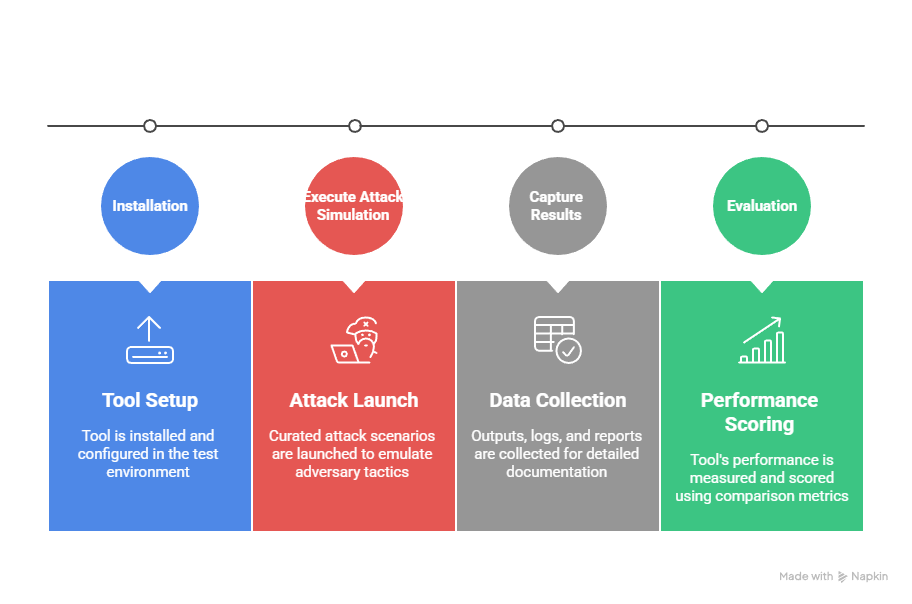
\includegraphics[width=1\linewidth]{figures/BAS-Testing Procedure - visual.png}
    \caption{Testing Procedure}
    \label{fig:Testing_Procedure}
\end{figure}

\noindent Figure~\ref{fig:Testing_Procedure} outlines the systematic four-phase methodology employed to evaluate the BAS tools. The process proceeds sequentially through: (1) Tool Setup, involving the installation and configuration of the test environment; (2) Attack Launch, where curated scenarios based on MITRE ATT\&CK are executed to emulate adversary tactics; (3) Data Collection, which captures comprehensive logs and tool outputs; and (4) Performance Scoring, where the gathered data is analyzed against six defined metrics to derive a final comparative assessment.
\end{itemize}
